\begin{figure}[ht]
\centering
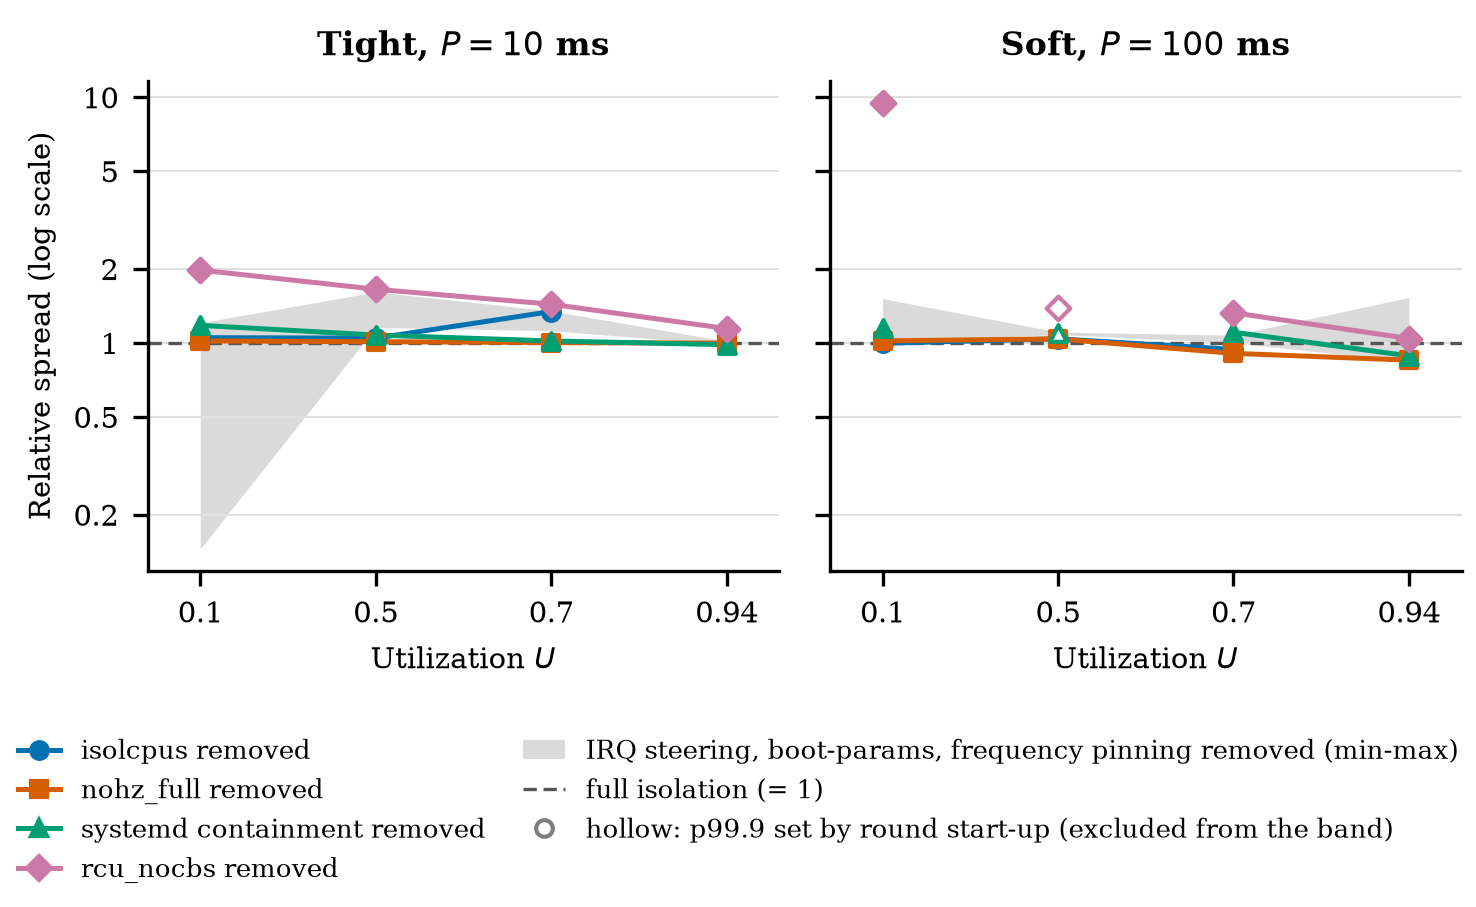
\includegraphics[width=\textwidth]{spread_multi-core.png}
\caption{Relative spread against utilization, multi-core: tail spread ($p_{99.9}/\mathrm{median}$ of the response time) of the configuration divided by that of full isolation (dashed line, 1), for the 10\,ms (left) and 100\,ms (right) period. Each line is one removed setting; the grey band spans the minimum and maximum of IRQ steering, the boot-params bundle and frequency pinning. Hollow points are cells whose $p_{99.9}$ is dominated by the start-up of the rounds: at least a quarter of the jobs above it are among the first five retained jobs of a round, in the configuration or in full isolation (the reference); they are left out of the band and not joined by a line. The first six jobs after every restart are excluded. The vertical axis is logarithmic. SMT enabled is not drawn: it shifts the whole distribution, including the median, so a tail-to-median ratio cannot show its effect (see Table~\ref{tab:rq1-multi-core} and the heatmap).}
\label{fig:rq1-spread-multi-core}
\end{figure}
